\documentclass[11pt,a4paper]{article}
\usepackage[utf8]{inputenc}
\usepackage[english]{babel}
\usepackage[T1]{fontenc}
\usepackage{amsmath}
\usepackage{amsfonts}
\usepackage{amssymb}
\usepackage{graphicx}
\usepackage{array}
\usepackage{multirow}
\usepackage[left=2cm,right=2cm,top=2cm,bottom=2cm]{geometry}
\author{Guillem Tocabens}
\title{First measurements}
\begin{document}

\section{Scanning the prototype detector}

%What is that detector ??? Add a part that describes this new prototype !

\subsection{Overall setup}

The global setup uses three detectors: two scintillator detectors, placed on the sides (black squared boxes on the picture, Figure \ref{Setup}) and one semi conductor detector - hyperpure germanium detector - below the collimated source (grey cylinder on the picture). The source is placed on the top lead brick which contains a hole in the middle to collimate the radioactive source. In that position, the source is 97mm from the top of the crystal, which is 5mm from the top of the cryostat (grey cylinder), and collimated in a 5mm hole through an 80mm lead brick. the source is covered by a little lead brick and the setup is shielded by lead to avoid propagation of gamma radiation away from the setup (see Figure \ref{Setup_front}).

\begin{figure}[!h]
\centering
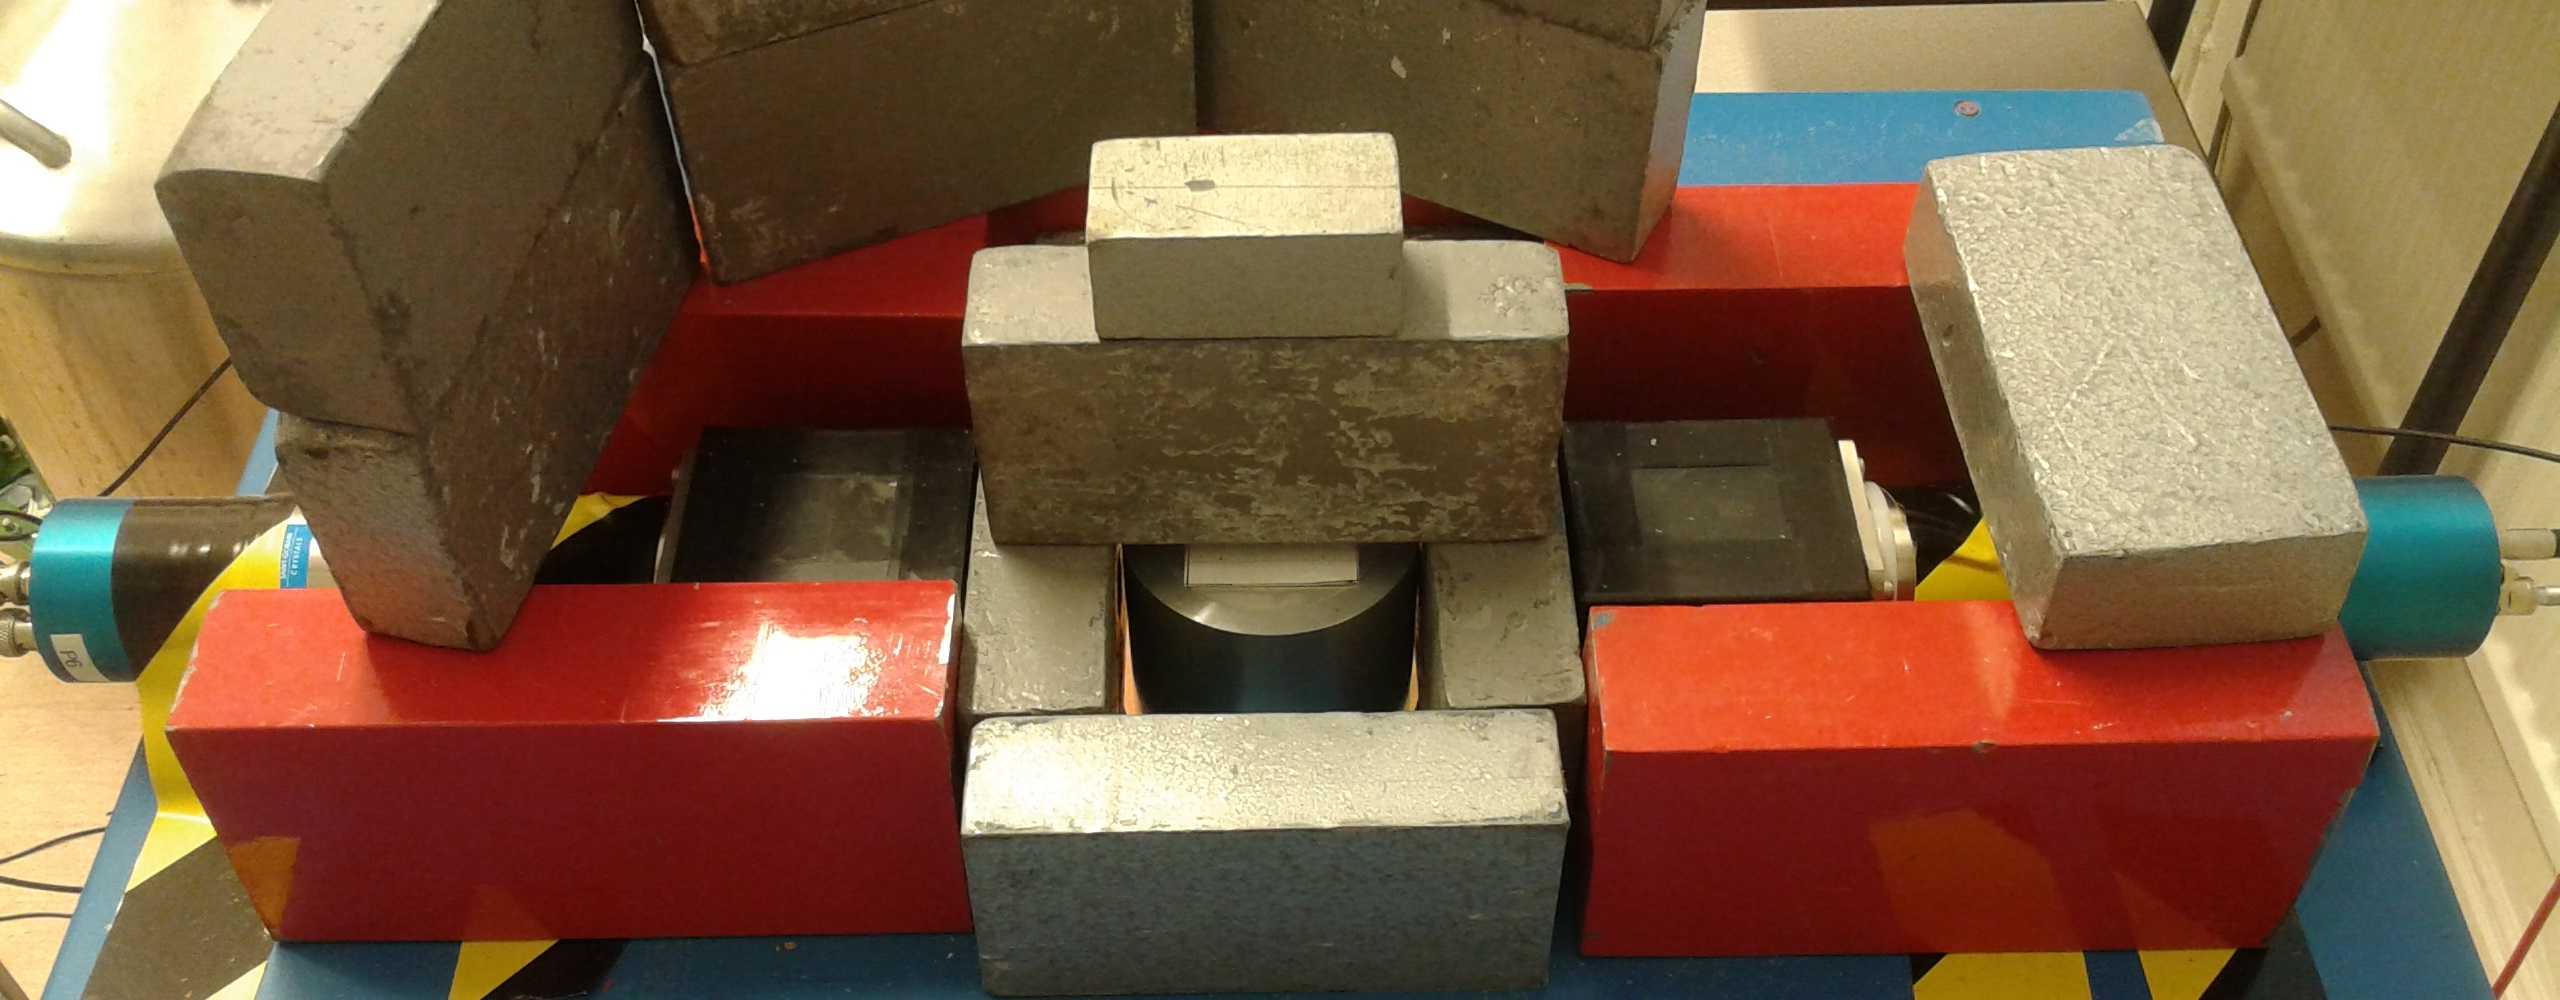
\includegraphics[scale=0.15]{New_setup_back.jpg}
\caption{Back of the original setup. The scintillator detectors are the black squared boxes on the sides of the germanium detector, placed in a cryostat (grey cylinder in the middle).}
\label{Setup}
\end{figure}

\begin{figure}[!h]
\centering
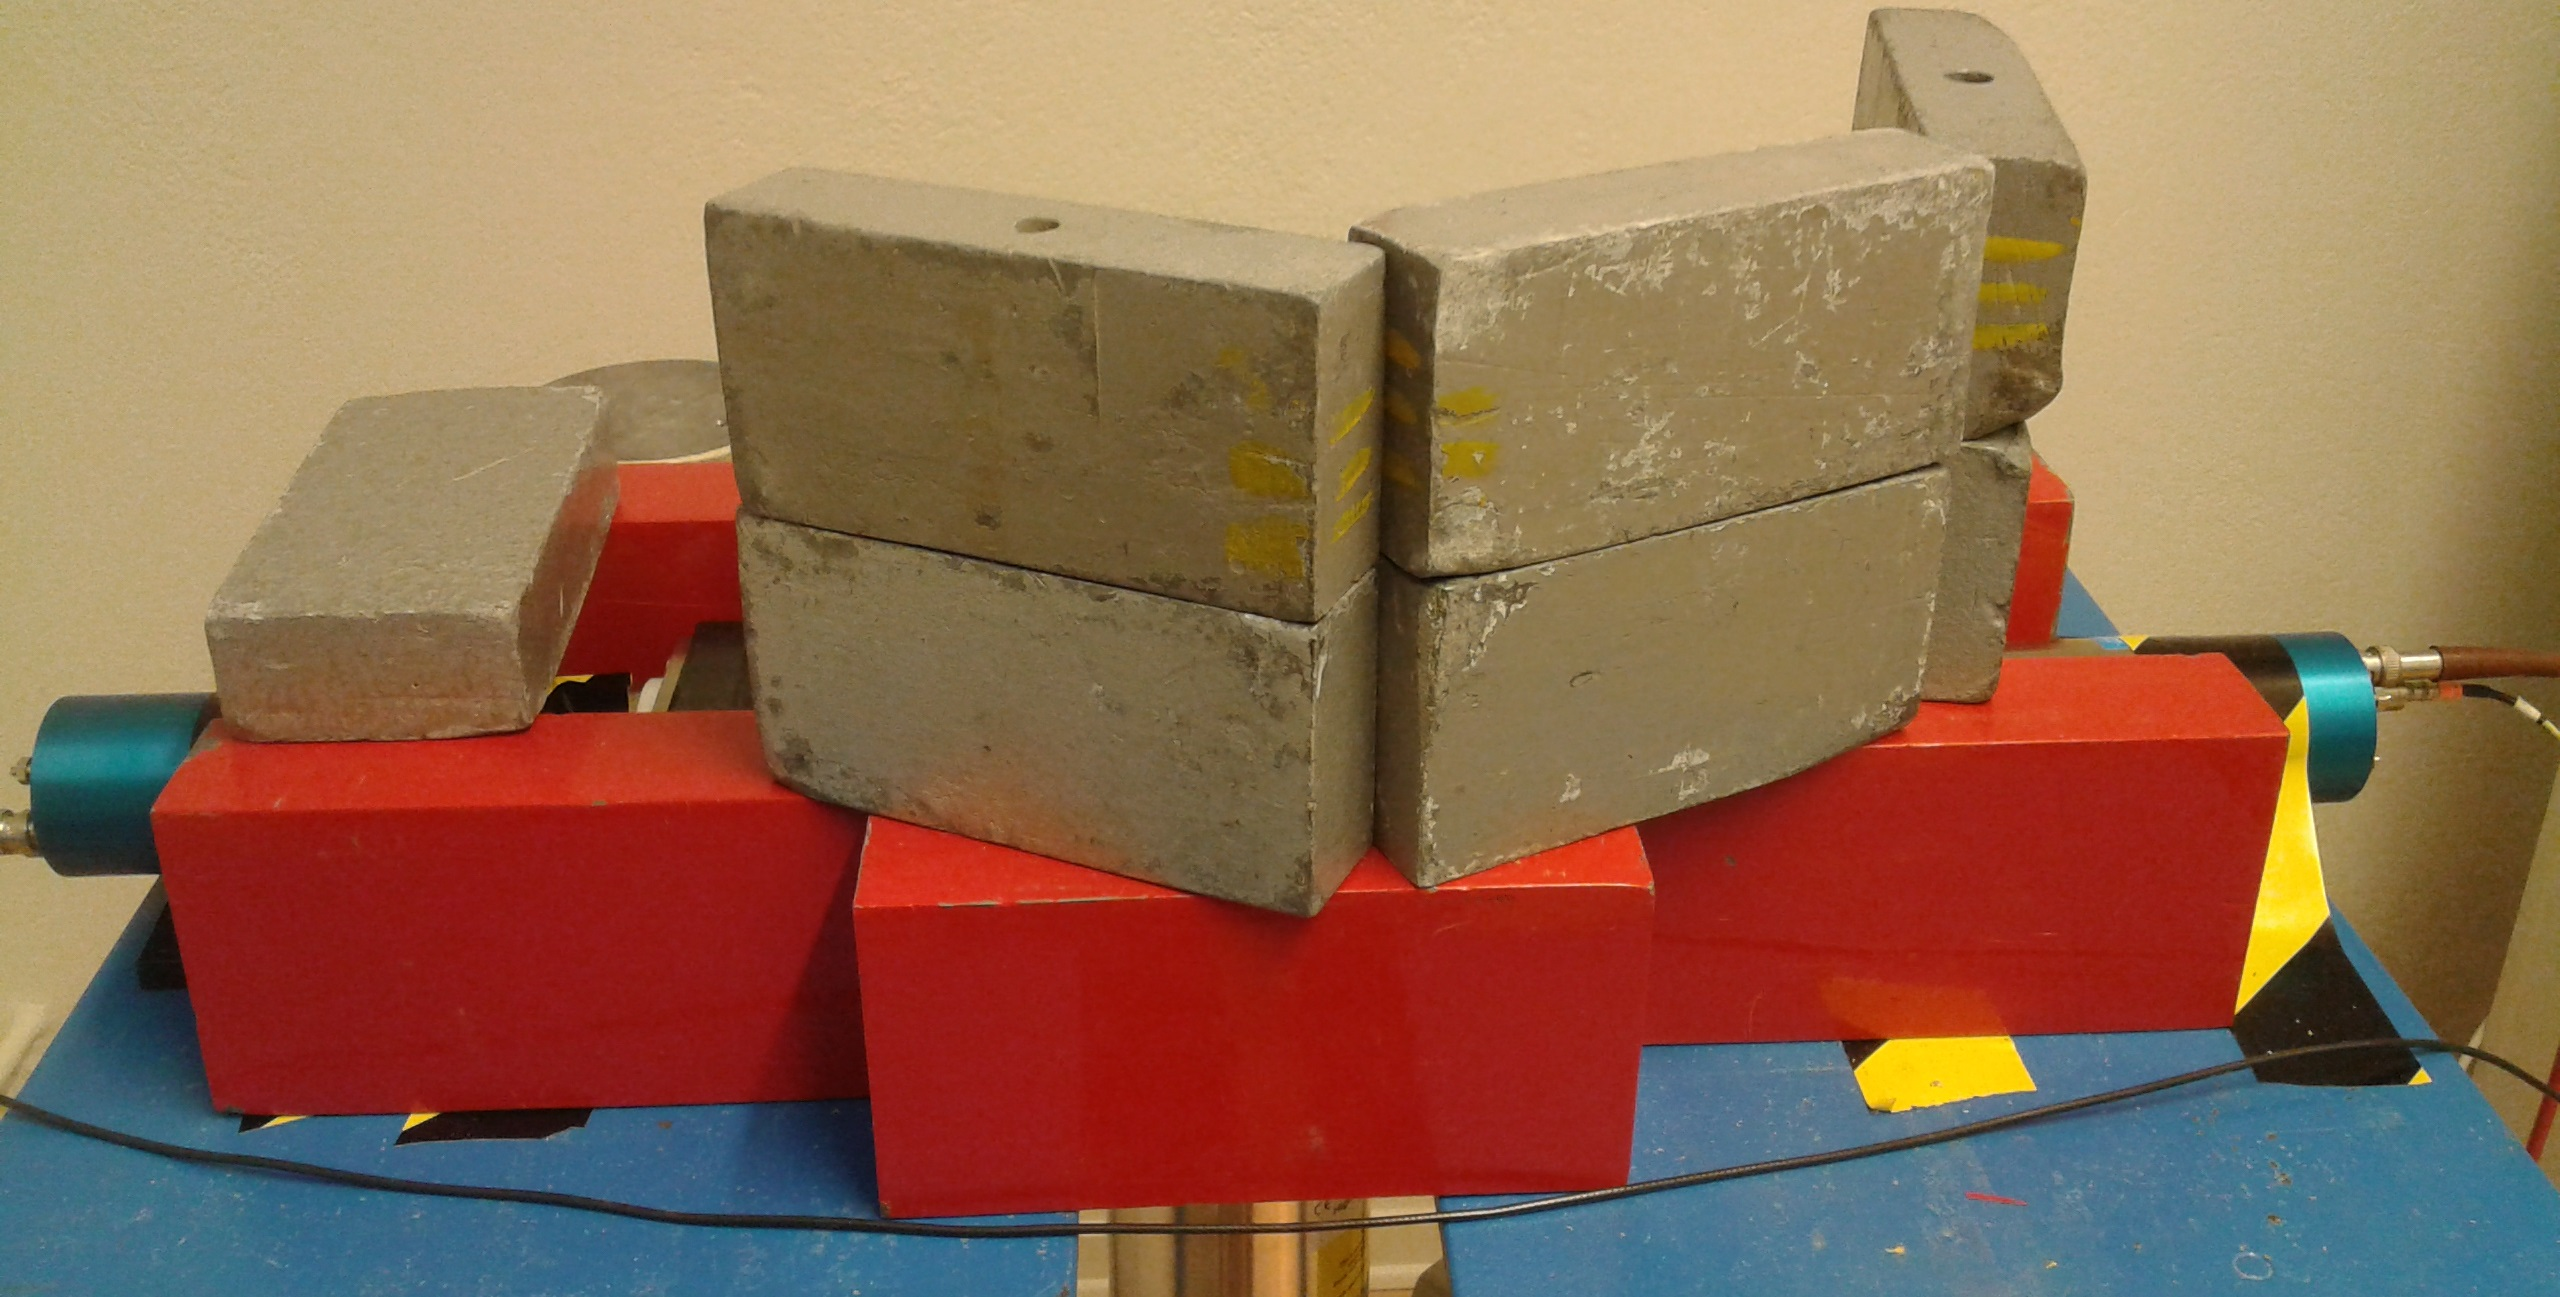
\includegraphics[scale=0.15]{New_setup_front.jpg}
\caption{Front side of the original setup (with the lead shielding).}
\label{Setup_front}
\end{figure}

\subsection{Process of measurement}

For this first set of measurements, we did not use the scintillator detectors but only the germanium detector. The goal of this experiment was to determine some properties of the detector depending on the location of the collimated source such as the resolution of the crystal. Therefore, we collimated the source in five different places on the top of the crystal: one measurement was performed with the collimator in the center of the crystal surface, and four were performed with the collimator in the corners of the crystal surface. The scanning went as described below (see scheme Figure \ref{scan}) and we used two different cobalt sources: one of $^{60}$Co and one of $^{57}$Co (the decay schemes are shown in Figure \ref{decayCos}).

\begin{figure}[!h]
\centering
\includegraphics[scale=0.6]{scan.png}
\caption{Scheme of the top of the germanium crystal and how it was scanned. Each circle represents a position of the collimated source to which we associate a number (distances are in mm).}
\label{scan}
\end{figure}

\begin{figure}[!h]
\centering
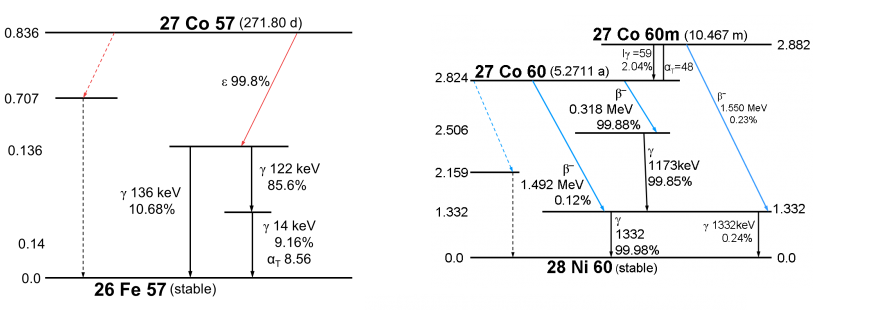
\includegraphics[scale=0.9]{Cos_decays.png}
\caption{Decay schemes of $^{60}$Co and $^{57}$Co.}
\label{decayCos}
\end{figure}

In the case of $^{60}$Co, the source was held in one of the positions until the net area of the studied peak (peak at 1332keV) contained at least 100~000 counts. The $^{57}$Co source being way less active, the measurement was stoped when the net area of the studied peak (peak at 122keV) contained around 1~000 counts.

The calibration was done using the source of $^{60}$Co and collimating it in the middle of the crystal to get a reference and study an eventual deviation in energy. For this purpose we used the two peaks present in the spectrum of $^{60}$Co and associated to each of them a channel in the 8192 channels that the multichannel analyzer contains. The result of the calibration is shown in Figure \ref{calib} with the equation of the linear fit. The data was then analyzed using a Python program to fit the peaks in the spectra with Gaussians (the code is given in appendix).

\begin{figure}[!h]
\centering
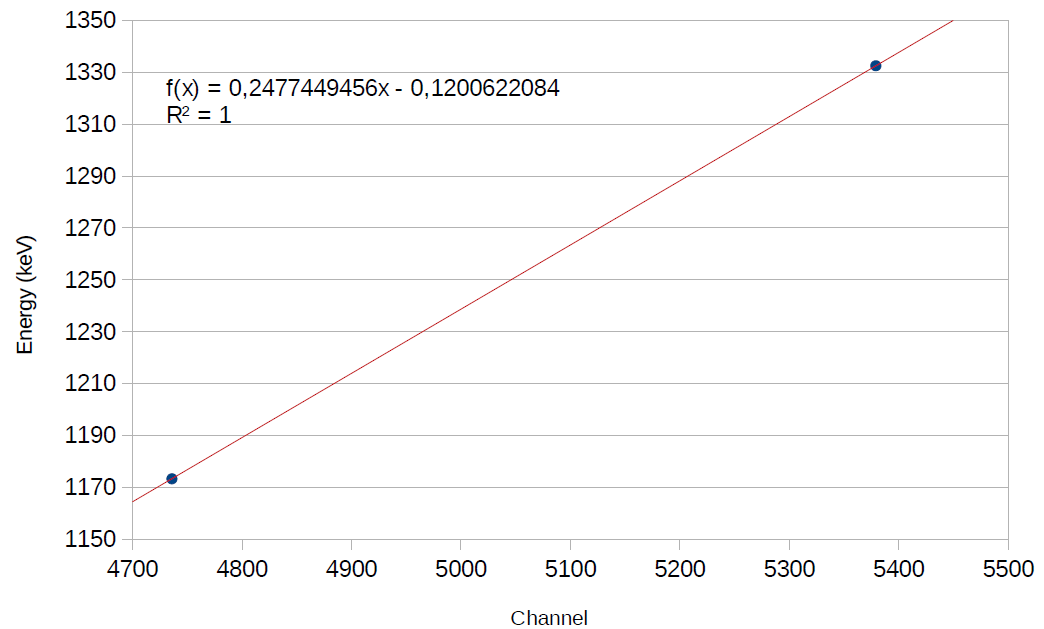
\includegraphics[scale=0.6]{calibration.png}
\caption{Calibration plot representing energy as a function of channel number, using the two peaks of $^{60}$Co spectrum.}
\label{calib}
\end{figure}

\subsection{Electronics}

%Do a beter picture (only with the two modules ?)
\begin{figure}[!h]
\centering
\includegraphics[scale=0.15]{electro1.png}
\caption{Picture of the electronics used in this measurements. The two modules that were used are the two first on the left (red arrow) and, from left to right, are the high voltage supply and the amplifier.}
\label{electro1}
\end{figure}

For this set of measurements, we did not use the scintillator detectors or the coincidence setup, thus the electronics are relatively simple. The detector is alimented by a high voltage supply which delivers a bias voltage (negative) of 5000kV, necessary to the well-functionning of the crystal. After going through a preamplifier (in the crystal), the signal is send to an amplifier that also shapes it. It is then digitized by a multichannel analyzer and send to the computer that collects the data using the Maestro software. Both the high voltage supply and the amplifier are NIM modules and are placed in a NIM crate, represented on Figure \ref{electro1}.

%What could we add here ?

\subsection{Results and analysis}

%Add stuff here ? More explanations maybe ?

For each of the position of interest, we collected the data and used the Python program to treat it. We looked at the resolution of the detector, given by the full width at half maximum (FWHM), along with the shape of the peak, emphasized by the ratios between the full width at tenth and fifteenth maximum and the FWHM. All these results are shown in the two tables below, both for the $^{60}$Co and $^{57}$Co source (Figure \ref{recap}).

\begin{figure}[!h]
\centering
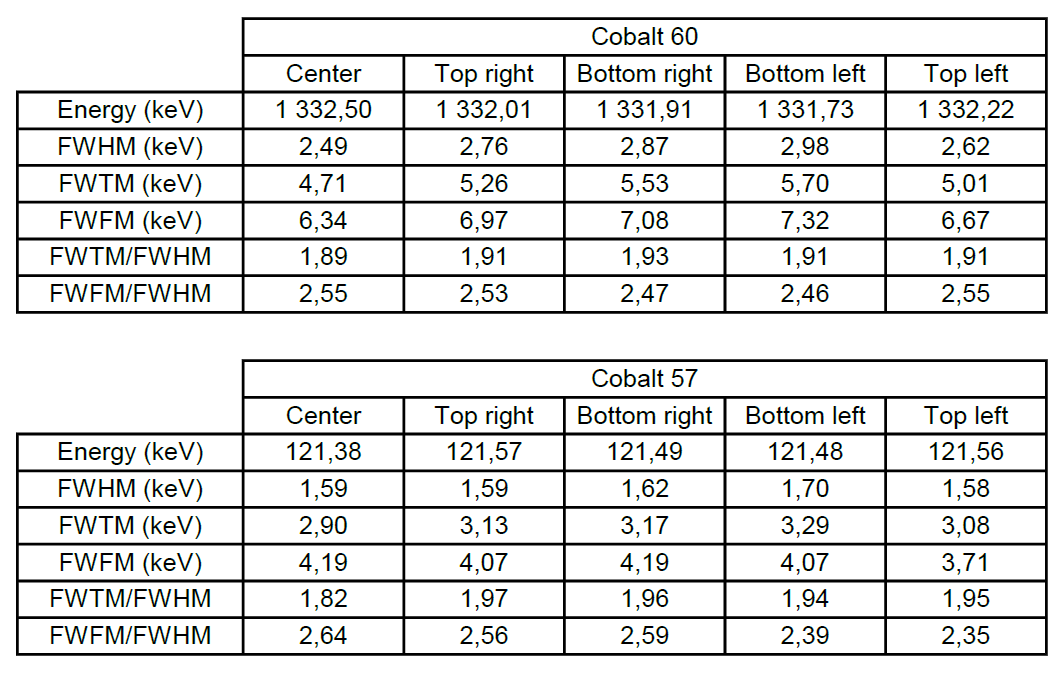
\includegraphics[scale=0.7]{Scan_Cos.png}
\caption{Recapitulative tables of the obtained results using the $^{60}$Co and $^{57}$Co sources ($^{60}$Co calibration).}
\label{recap}
\end{figure}

The very first thing we can notice is that the peaks are not present at the same energy in all of the spectra. Indeed, while the calibration was done using the spectrum of $^{60}$Co collimated in the center of the crystal, this measure is exactly where we expect it to be looking in the literature (see Figure \ref{decayCos}). But then, if we take another measurement, where the source was collimated on a corner, there is a shift in energy up to 0.8keV. If we look at the energies for the $^{57}$Co source, we can see that they are not exactly what we expect (the usual value of this peak is 122.06keV). This can be explained by the fact that the calibration was performed using the two peaks of the $^{60}$Co source, and thus no energy peak in the low-energy zone. A second set of measurements was done using the two cobalt sources as a calibration (see Figure \ref{calib2}), both collimated in the center of the crystal surface. This second set of measurements gives very similar results in the right part of the spectrum (for $^{60}$Co), but different energy and resolution values in the left part of the spectrum (for $^{57}$Co), see Figure \ref{recap2}.

%WARNING: shift is in the range of the resolution, is it really relevant to notice ???

If we now look at the resolution measurements, we can point out some differences between the center and the corners (up to 0.5keV) and it seems that when we collimate the source in the center, we obtain a better resolution than while collimating it in a corner, at least when looking at the values for the peak at 1332.5keV of $^{60}$Co. Indeed, the values are quiet close for the $^{57}$Co source, either collimating the source in the center of the crystal or in the corners. If we now compare these values with the resolution values given by Canberra for the prototype detector, we can see that they are quiet close to what we obtained for the $^{60}$Co source, but way smaller for the $^{57}$Co source, around twice as thin as what we measured. This huge difference with our values can be explained by the $^{57}$Co source we used: the source was too weak and we could not get a net area of 100~000 counts under the peak as they did in Canberra. Thus, these values were measured with a net area of around 1~000 counts under the peak and it is normal that they differ a lot as the peak was not pointing as high over the background as it should have.

Finally, if we look at the symmetry ratios, being defined as \textit{"is the peak really looking as a Gaussian ?"}, we can notice that they are pretty close to the theoretical values (values for a real Gaussian) as those are:

\begin{equation}
\dfrac{FWTM}{FWHM} = 1.82 \text{ and } \dfrac{FWFM}{FWHM} = 2.38
\end{equation}
Again, for the $^{57}$Co source, it may not make a lot of sense to look at those values, as the peak is not large enough to be analyzed in a very proper way, but the values obtained for the $^{60}$Co source are closer to the theoretical values than the values given by Canberra, meaning that the peaks we obtained on the spectra have a better Gaussian shape.

\begin{figure}[!h]
\centering
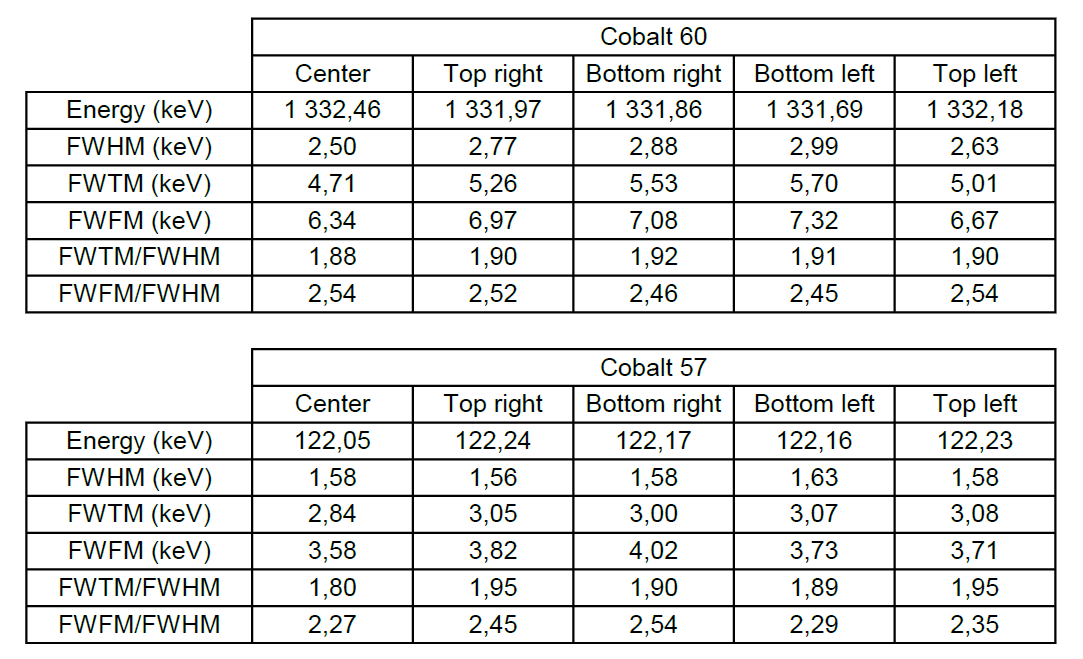
\includegraphics[scale=0.7]{Scan_Cos_2.png}
\caption{Recapitulative tables of the obtained results using the $^{60}$Co and $^{57}$Co sources ($^{60}$Co and $^{57}$Co calibration).}
\label{recap2}
\end{figure}

\begin{figure}[!ht]
\centering
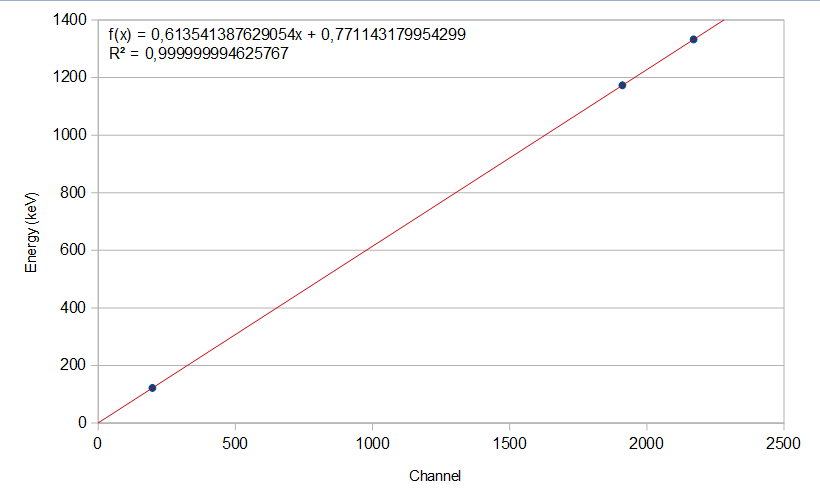
\includegraphics[scale=0.9]{Calibration_2.png}
\caption{Calibration plot representing energy as a function of channel, using the two peaks of $^{60}$Co and the 122keV peak of $^{57}$Co.}
\label{calib2}
\end{figure}

\end{document}